\documentclass[conference]{IEEEtran}
\IEEEoverridecommandlockouts
% The preceding line is only needed to identify funding in the first footnote. If that is unneeded, please comment it out.
\usepackage{cite}
\usepackage{amsmath,amssymb,amsfonts}
\usepackage{algorithmic}
\usepackage{graphicx}
\usepackage{textcomp}
\usepackage{xcolor}
\def\BibTeX{{\rm B\kern-.05em{\sc i\kern-.025em b}\kern-.08em
    T\kern-.1667em\lower.7ex\hbox{E}\kern-.125emX}}

\begin{document}

\title{Pengembangan Program Microwave dengan Pendekatan Computational Thinking
}

\author{
\IEEEauthorblockN{Marcheline Fanni Hidayat Putri\IEEEauthorrefmark{1}, Angela Livia Arumsari\IEEEauthorrefmark{2}, Miralistya Cahya Fatimah\IEEEauthorrefmark{3}}
\IEEEauthorblockA{\textit{KU1102 21-Introduction to Computation}\\\textit{School of Electrical Engineering and Informatics} \\
\textit{Institut Teknologi Bandung}\\
Bandung, Indonesia \\
Email: \IEEEauthorrefmark{1}16521117@mahasiswa.itb.ac.id, \IEEEauthorrefmark{2}16521177@mahasiswa.itb.ac.id, \IEEEauthorrefmark{3}16521207@mahasiswa.itb.ac.id}\\
}
\maketitle

\section{PENDAHULUAN}
Teknologi adalah suatu hal yang sangat membantu dan mengambil peran dalam kehidupan manusia. Hal ini dikarenakan teknologi dapat bekerja secara efektif dan efisien.
Dibalik teknologi yang bagus tersebut, pastinya terdapat suatu pemrograman yang telah dirancang sedemikian rupa seehingga menghasilkan program yang berjalan dengan tepat dan menghasilkan teknologi
yang baik pula. Pada zaman yang sudah sangat maju ini, segala aspek dalam kehidupan manusia tidak dapat 
dipisahkan dari teknologi, artinya, dalam kehidupan manusia, kita memanfaatkan banyak program yang telah dirancang dengan baik. Salah satu contoh sederhananya adalah Microwave.
Manusia selama ini sering memanfaatkan microwave dalam kehidupan sehari-harinya. Teknologi ini sangat membantu dan memudahkan kita, tanpa kita mengetahui bagaimana sebenarnya pemrograman pada microwave.
Maka dari itu, kelompok kami akan mencoba membuat dan membahas pemrograman pada microwave.

Tujuan dari pengembangan program microwave ini, diantaranya:
\begin{itemize}
    \item Melatih kemampuan membuat suatu program.
    \item Mengasah kemampuan computational dan algorithmic thinking.
    \item Mampu berpikir secara kritis mengenai keberjalanan suatu program dari suatu teknologi yang kita manfaatkan sehari-hari.
    \item Meningkatkan kerjasama antar anggota kelompok dan saling bertukar pikiran sehingga menambah ilmu dan wawasan.
\end{itemize}


\section{KONSEP MICROWAVE}

\subsection{Pengertian}
Microwave merupakan sebuah alat elektronik yang secara umum berfungsi untuk 
menghangatkan makanan dengan memanfaatkan listrik dan radiasi gelombang mikro. 
Gelombang mikro yang dimanfaatkan oleh microwave biasanya memiliki frekuensi 2.450 MHz 
dan panjang gelombang sekitar 12,24 cm. Molekul air, gula, dan lemak dalam makanan bisa 
menyerap gelombang mikro tersebut. 

\subsection{Sistem Kerja}
Microwave memiliki magnetron yang dirancang untuk memanfaatkan energi dalam microwave. 
Aliran listrik disuplai ke tabung magnetron untuk menciptakan energi gelombang mikro. Gelombang mikro ini 
menembus area pemanasan saat dimulainya proses awal dalam microwave.

Gelombang mikro tidak bisa menembus dinding logam microwave, tapi dapat menembus materi tertentu, seperti kaca, 
porselen, dan kertas yang menjadi bahan dasar peralatan memasak yang aman digunakan untuk microwave. 
Gelombang mikro tidak memanaskan peralatan masak, meski lambat laun barang-barang tersebut mendapatkan panas yang 
berasal dari makanan.

\subsection{Fitur-Fitur pada Microwave}

\begin{enumerate}
\item[1)]Manual
adalah salah satu pilihan mode pada microwave dengan pilihan suhu dan waktu menyesuaikan dengan keinginan pengguna. 
 Mode ini dibebaskan untuk semua jenis makanan.

\item[2)]Defrost
    \begin{itemize}
    \item Auto Defrost adalah salah satu pilihan mode pada microwave untuk melunakkan meat, poultry, fish, atau bread. Pengguna perlu menentukan 
    terlebih dahulu kategori makanan yang akan diproses pada microwave, lalu pengguna juga akan diminta untuk memasukkan data berat bahan yang akan 
    diproses agar microwave dapat menentukan lama waktu pemrosesan secara otomatis. Level daya pada mode ini telah diatur secara otomatis sehingga tidak 
    diperlukan masukan mode dari pengguna.
    \item Quick Defrost adalah salah satu pilihan mode pada microwave untuk melunakkan 0,5 kg daging cincang beku dengan sangat cepat. Pada mode ini pengguna tidak 
    perlu lagi menentukan lama waktu proses dan juga suhu yang diaplikasikan pada microwave karena suhu dan waktu akan ditentukan secara otomatis. Proses ini 
    menyediakan waktu pendiaman untuk membiarkan bagian tengah melunak
    \end{itemize}

\item[3)]Reheat
adalah salah satu mode microwave untuk melakukan pemanasan atau penghangatan makanan berdasarkan waktu yang akan ditentukan oleh pengguna, 
dengan batasan waktu maksimal yaitu 30 menit. Pada fitur ini pengguna tidak akan diminta untuk memasukkan suhu atau level daya, karena sudah diatur secara otomatis, 
yaitu pada daya High level.

\item[4)]Quick Action
adalah salah satu mode pada microwave yang dapat dipilih dengan cepat. Setting suhu dan lama waktu pemrosesan telah diaplikasikan secara otomatis berdasarkan pilihan 
kategori makanan dari pengguna. Kategori makanan yang tersedia yaitu Veggies, Bread, Meat, Fish, Soup, dan Beverage.
\end{enumerate}

\subsection{Dekomposisi}

\begin{figure}[htbp]
    \centering
    \def\svgwidth{\columnwidth}
    \centerline{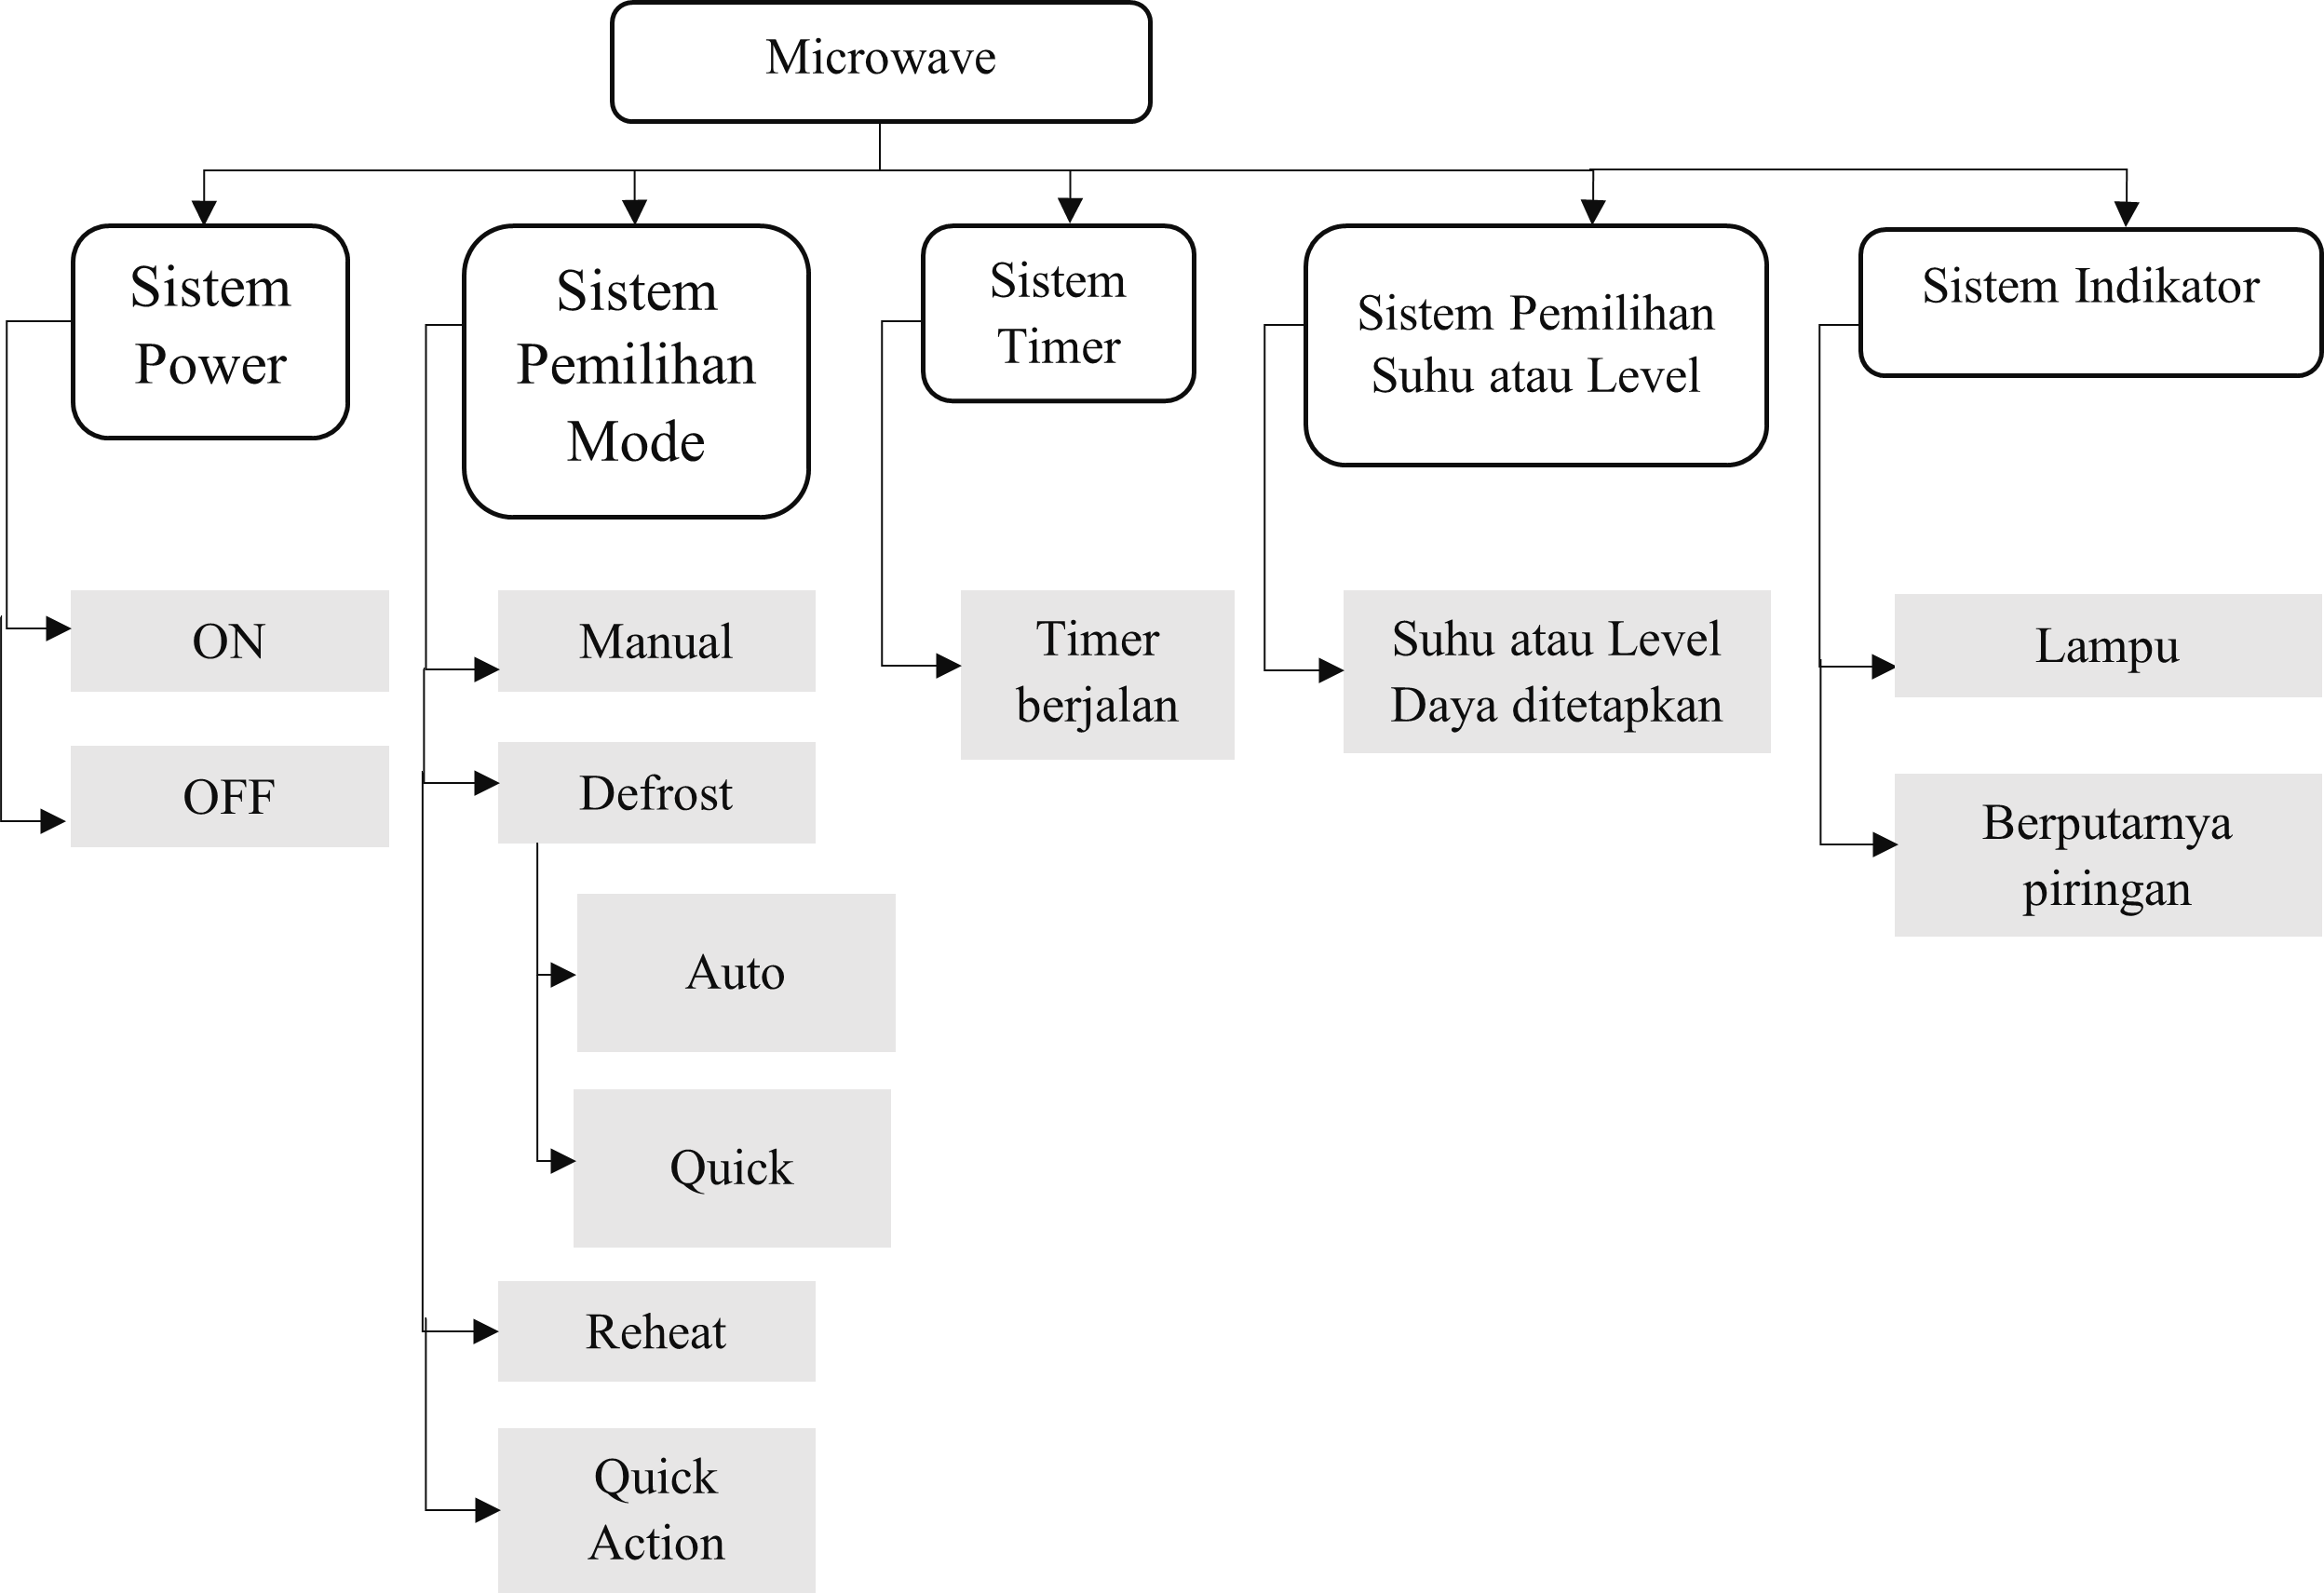
\includegraphics[scale=0.45]{dekomposisi.png}}
    \caption{Dekomposisi Microwave}
    \label{fig1}
\end{figure}

\section{PROGRAM MICROWAVE}

\subsection{Deskripsi}

\begin{enumerate}
\item[1)] Microwave :\\
Saat pertama kali dijalankan, program microwave akan menampilkan empat pilihan mode microwave yaitu \textit{manual, defrost, reheat, dan quick action.} Pengguna akan diminta 
untuk \textit{input mode} yang dipilih dalam bentuk \textit{integer} dengan ketentuan angka 1 untuk memilih mode manual, angka 2 untuk mode defrost, angka 3 untuk mode reheat, 
dan angka 4 untuk mode quick action. Setelah itu, program akan melakukan \textit{proses mode} microwave sesuai pilihan pengguna. Jika bilangan yang dimasukkan bukan merupakan angka 1, 2, 3, atau 4, 
maka program akan memberikan \textit{output} tulisan “Mode tidak tersedia!” dan akan meminta pengguna untuk \textit{input} pilihan modenya kembali. Program microwave ini menggunakan dua modul, yaitu modul os 
dan modul time. Modul os digunakan untuk membersihkan terminal setiap kali pergantian menu agar tampilan program lebih rapi. Modul time digunakan untuk menjalankan fungsi timer (hitung mundur) 
selama proses pemanasan sesuai mode yang telah dipilih. Setelah proses mode selesai dijalankan, pengguna akan diminta untuk \textit{input integer}, 1 untuk menggunakan microwave lagi, yaitu pengguna akan 
kembali ke tampilan empat pilihan mode microwave di awal atau \textit{input integer} 2 untuk mematikan microwave.
 
\item[2)] Manual : \\
Ketika pengguna memilih mode manual, pengguna akan diminta untuk \textit{input suhu} dalam satuan Celcius. Suhu yang dimasukkan harus berada di rentang 30 hingga 300. Bila tidak sesuai, maka program akan meminta 
pengguna untuk \textit{input ulang suhu} di antara 30 dan 300 derajat Celcius. Setelah proses input suhu selesai, program akan meminta \textit{input waktu} berupa menit dan detik dalam bentuk bilangan bulat bukan negatif. 
Program akan berjalan jika menit yang dimasukkan kurang dari 30 menit. Jika input dari pengguna sudah sesuai, maka program akan melakukan \textit{proses} yaitu menghitung waktu dalam bentuk detik untuk menjalankan timer (mengalikan 
menit yang dimasukkan dengan 60 lalu menambahkannya dengan detik yang telah dimasukkan). Setelah itu, program akan menampilkan menit, detik, dan suhu yang akan dijalankan. Sebelum memulai proses, pengguna akan diminta 
untuk \textit{input integer} 1 untuk memulai, 2 untuk kembali ke mode manual, atau 3 untuk kembali ke pilihan mode. Jika pengguna memilih angka 1, maka program akan mulai menjalankan \textit{proses} hitung mundur sesuai dengan waktu 
yang telah dimasukkan dengan bantuan modul time. Setelah hitung mundur selesai, program akan memberikan \textit{output} “Program Selesai!” dan meminta pengguna untuk \textit{input} angka 1 untuk kembali ke mode pilihan mode atau 2 untuk 
mematikan microwave.

\item[3)] Defrost :\\
Ketika pengguna memilih mode Defrost, pengguna akan diberikan dua pilihan, yaitu auto defrost dan quick defrost. Pengguna akan melakukan \textit{input} angka 1 untuk auto defrost atau angka 2 untuk quick defrost. Program akan melakukan proses 
berdasarkan input pengguna. Jika input tidak sesuai, maka program akan melakukan \textit{proses} looping untuk meminta masukan opsi defrost yang tersedia. 

Jika pengguna melakukan \textit{input} angka 1 saat memilih opsi defrost, maka program akan menjalankan opsi auto defrost. Pada opsi auto defrost, program telah menyimpan 4 array, yaitu bahan [“Meat”, “Poultry”, “Fish”, “Bread”], menit yaitu [6, 5, 5, 3], detik yaitu [25, 15, 10, 50],
dan level yaitu [“HIGH”, “HIGH”, “HIGH”, “LOW”]. Program akan menampilkan \textit{output} bahan-bahan yang tersedia dan menerima \textit{input} bilangan bulat dari pengguna sesuai dengan indeks dari bahan yang dipilih ditambah 1. Program akan melakukan \textit{proses} kondisional berdasarkan input 
yang diterima serta melakukan looping hingga input sesuai dengan bahan yang tersedia. Setelah itu, program akan menerima \textit{input berat} berupa bilangan riil. Berat yang diinput haruslah minimal 0.1 kg dan maksimal 4 kg. Apabila tidak sesuai, pengguna 
akan diminta untuk mengulang input tersebut. Kemudian, program akan memproses menit dan detik berdasarkan bahan dan beratnya. Program akan menampilkan \textit{output menit, detik, dan level} defrost yang akan dijalankan. Pengguna akan memasukkan \textit{input} 
angka 1 untuk memulai, 2 untuk kembali ke mode defrost, atau 3 untuk kembali ke pilihan mode. Jika pengguna memasukkan angka 1, maka \textit{proses} hitung mundur akan berjalan sesuai dengan variabel t dengan bantuan modul time. Setelah hitung mundur selesai. 
program akan menampilkan \textit{output} “Program Selesai!” dan meminta pengguna untuk memasukkan \textit{input} angka 1 untuk kembali ke mode pilihan mode atau 2 untuk mematikan microwave.

Jika pengguna memasukkan \textit{input} angka 2 saat memilih opsi defrost, maka program akan menjalankan opsi quick defrost. Pada opsi ini, program secara otomatis menetapkan waktu pemanasan selama 5 menit dan 30 detik dengan level HIGH. Waktu 
tersebut kemudian akan dikonversi menjadi detik. Program akan menampilkan \textit{output menit, detik, dan level} pemanasan ulang yang akan dijalankan. Pengguna akan memasukkan \textit{input} angka 1 untuk memulai, 2 untuk kembali ke mode reheat, 
atau 3 untuk kembali ke pilihan mode. Jika pengguna memasukkan \textit{input} angka 1, maka \textit{proses} hitung mundur akan berjalan sesuai dengan waktu yang telah diubah ke detik dengan bantuan modul time. Setelah hitung mundur selesai. program 
akan menampilkan \textit{output} “Program Selesai!” dan meminta pengguna untuk memasukkan \textit{input} angka 1 untuk kembali ke mode pilihan mode atau 2 untuk mematikan microwave.


\item[4)] Reheat :\\
Ketika pengguna memilih mode reheat, pengguna akan diminta untuk \textit{input waktu} yaitu menit dan detik dalam bentuk bilangan cacah. Program akan melakukan \textit{proses} looping dan kondisional berdasarkan masukan yang diberikan 
oleh pengguna. Bila menit yang diinput lebih dari 30 menit atau bilangan menit dan/atau detik bukan merupakan bilangan cacah, maka pengguna akan diminta untuk \textit{input kembali} menit dan detik yang ingin dijalankan. Jika menit dan detik 
yang dimasukkan sudah sesuai, program akan menghitung total detik yang akan dijalankan, yaitu menit masukan dikali 60 lalu ditambahkan dengan detik masukan. Program akan memberikan \textit{output} menit dan detik waktu pemanasan ulang yang akan dijalankan. 
Pengguna akan diminta untuk \textit{input} angka 1 untuk memulai, 2 untuk kembali ke mode reheat, atau 3 untuk kembali ke pilihan mode. Jika pengguna memasukkan angka 1, maka \textit{proses} hitung mundur akan berjalan sesuai dengan waktu yang telah 
diubah ke detik dengan bantuan modul time. Setelah hitung mundur selesai, program akan memberikan \textit{output} “Program Selesai!” dan meminta pengguna untuk \textit{input} angka 1 untuk kembali ke mode pilihan mode atau 2 untuk mematikan microwave.
 
\item[5)] Quick Action :\\
Pada mode Quick Action, program menyimpan 3 array berupa kategori [“Veggies”, “Bread”, ”Meat”, “Fish”, “Soup”, “Beverage”], menit [1, 0, 2, 1, 2, 1], dan detik [30, 45, 0, 30, 0 ,0]. Ketika pengguna memilih mode ini, program akan menampilkan \textit{output} 
pilihan kategori makanan, kemudian pengguna akan memasukkan \textit{input} angka yang menunjukkan pilihan kategorinya. Setelah itu, program akan memproses menit dan detik sesuai dengan indeks dari kategori yang telah dipilihnya. Pada mode ini, setiap kategori 
yang tersedia memiliki lama waktu yang berbeda-beda yang telah diatur secara otomatis, yaitu veggies (1 menit 30 detik), bread (0 menit 45 detik), meat (2 menit 0 detik), fish (1 menit 30 detik), soup (2 menit 0 detik), dan beverage (1 menit 0 detik). Lalu, menit dan 
detik tersebut akan dikonversi dan dijumlahkan dalam bentuk detik. Program akan menampilkan \textit{output} menit dan detik waktu pemanasan ulang yang akan dijalankan. Pengguna akan memberikan \textit{input} angka 1 untuk memulai, 2 untuk kembali ke mode quick action, atau 3 untuk 
kembali ke pilihan mode. Jika pengguna input angka 1, maka \textit{proses} dilaksanakan, yaitu hitung mundur akan berjalan sesuai dengan waktu yang telah diubah ke detik dengan bantuan modul time. Setelah hitung mundur selesai, program akan menampilkan \textit{output} 
“Program Selesai!” dan meminta pengguna untuk memberikan \textit{input} angka 1 untuk kembali ke mode pilihan mode atau 2 untuk mematikan microwave.
\end{enumerate} 

\subsection{Flowchart}

\begin{figure}[htbp]
    \centering
    \def\svgwidth{\columnwidth}
    \centerline{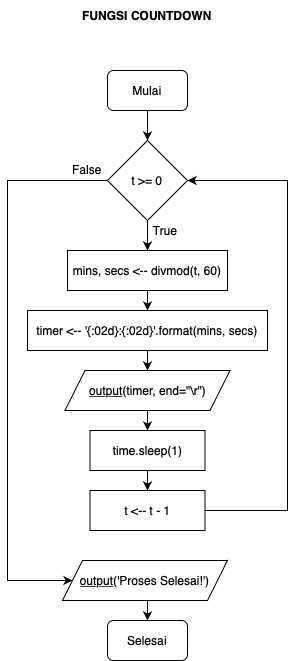
\includegraphics[scale=0.45]{Time.png}}
    \caption{Flowchart Fungsi Countdown}
    \label{fig2}
\end{figure}

\begin{figure}[htbp]
    \centering
    \def\svgwidth{\columnwidth}
    \centerline{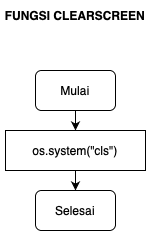
\includegraphics[scale=0.35]{Clearscreen.png}}
    \caption{Flowchart Fungsi Clearscreen}
    \label{fig3}
\end{figure}

\begin{figure}[htbp]
    \centering
    \def\svgwidth{\columnwidth}
    \centerline{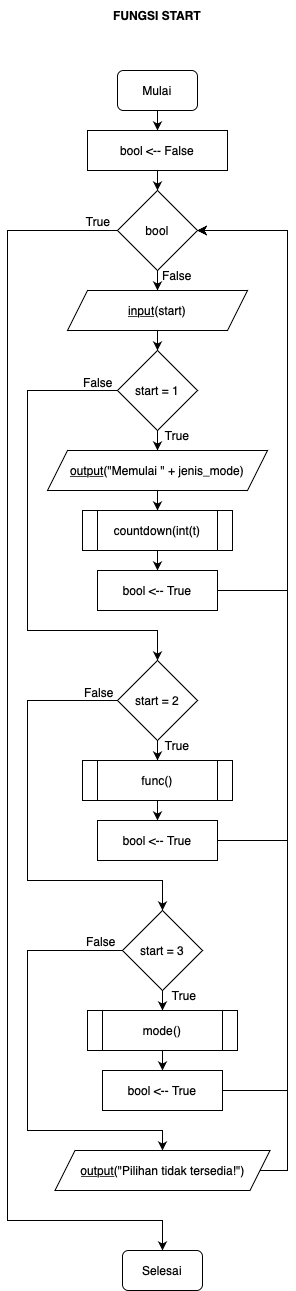
\includegraphics[scale=0.4]{Start.png}}
    \caption{Flowchart Fungsi Start}
    \label{fig4}
\end{figure}

\begin{figure}[htbp]
    \centering
    \def\svgwidth{\columnwidth}
    \centerline{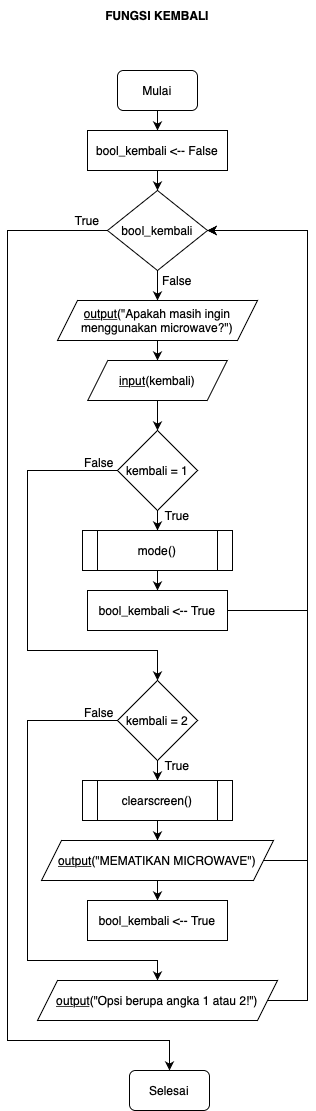
\includegraphics[scale=0.45]{Kembali.png}}
    \caption{Flowchart Fungsi Kembali}
    \label{fig5}
\end{figure}

\begin{figure}[htbp]
    \centering
    \def\svgwidth{\columnwidth}
    \centerline{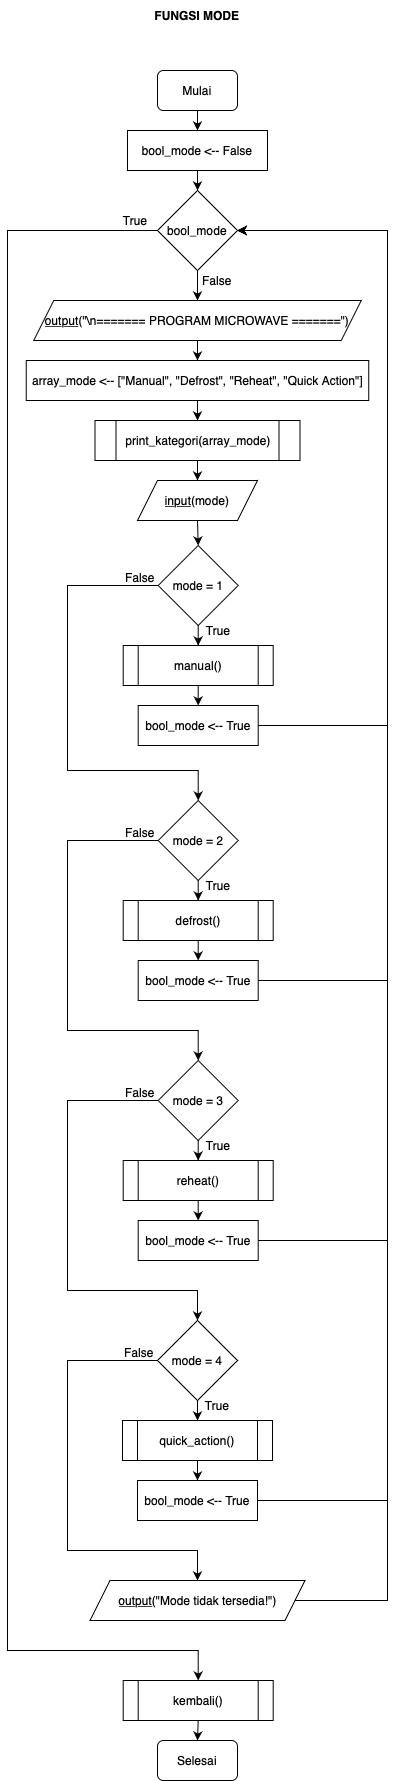
\includegraphics[scale=0.36]{Mode.png}}
    \caption{Flowchart Fungsi Mode}
    \label{fig6}
\end{figure}

\begin{figure}[htbp]
    \centering
    \def\svgwidth{\columnwidth}
    \centerline{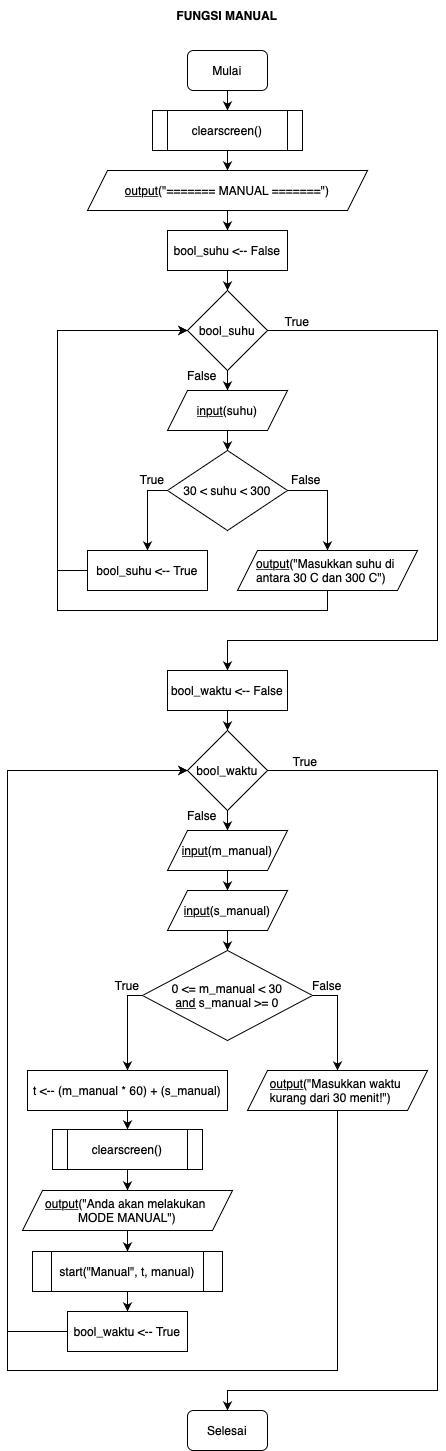
\includegraphics[scale=0.435]{Manual.png}}
    \caption{Flowchart Fungsi Manual}
    \label{fig7}
\end{figure}

\begin{figure}[ht]
    \centering
    \def\svgwidth{\columnwidth}
    \centerline{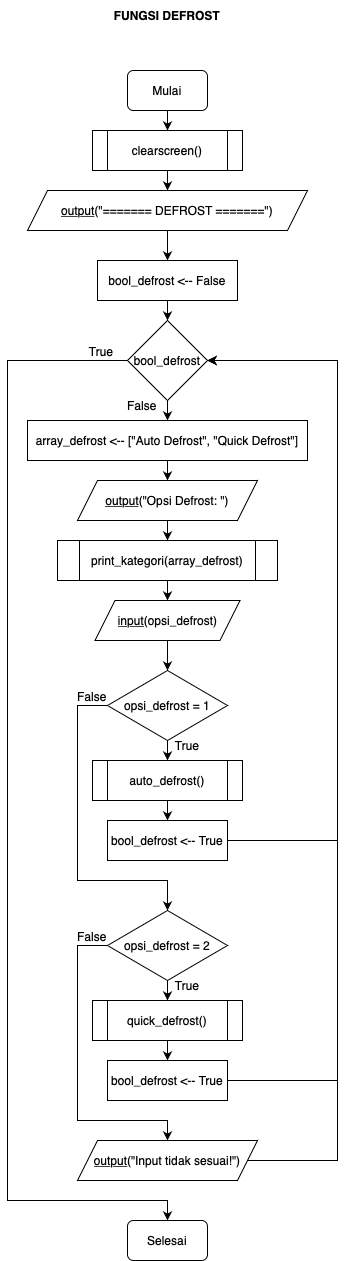
\includegraphics[scale=0.435]{Defrost.png}}
    \caption{Flowchart Fungsi Defrost}
    \label{fig8}
\end{figure}

\begin{figure}[htbp]
    \centering
    \def\svgwidth{\columnwidth}
    \centerline{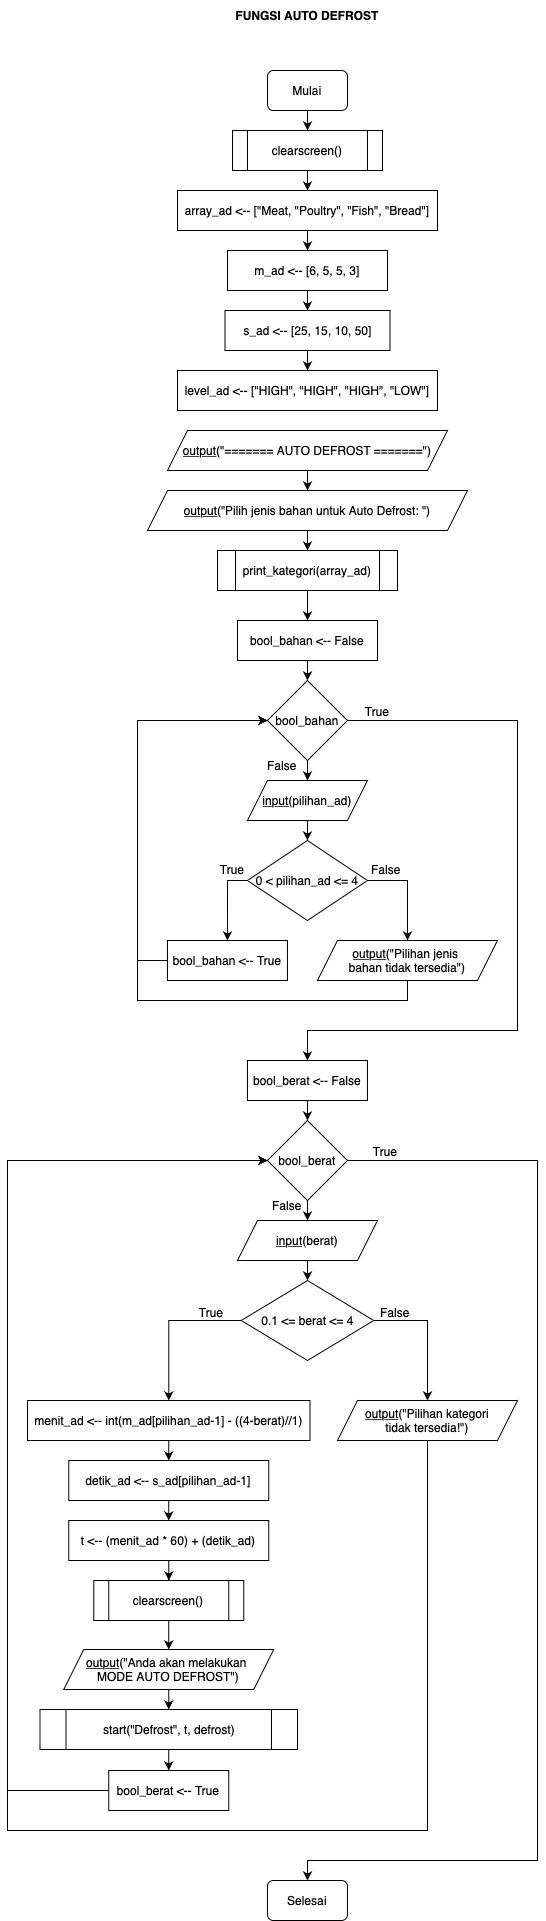
\includegraphics[scale=0.33]{AutoDefrost.png}}
    \caption{Flowchart Fungsi Auto Defrost}
    \label{fig9}
\end{figure}

\begin{figure}[htbp]
    \centering
    \def\svgwidth{\columnwidth}
    \centerline{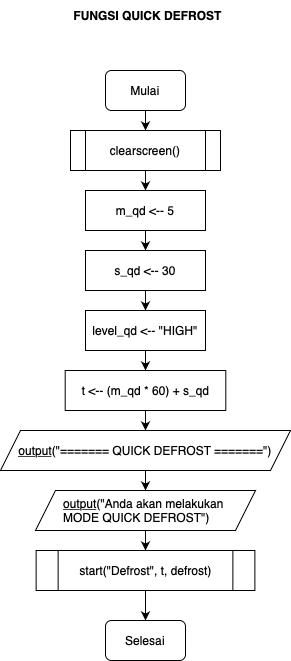
\includegraphics[scale=0.45]{QuickDefrost.png}}
    \caption{Flowchart Fungsi Quick Defrost}
    \label{fig10}
\end{figure}

\begin{figure}[htbp]
    \centering
    \def\svgwidth{\columnwidth}
    \centerline{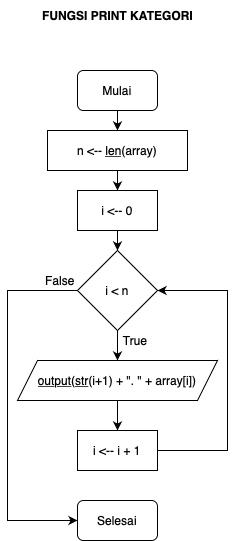
\includegraphics[scale=0.45]{PrintArray.png}}
    \caption{Flowchart Fungsi Print Kategori}
    \label{fig11}
\end{figure}

\begin{figure}[htbp]
    \centering
    \def\svgwidth{\columnwidth}
    \centerline{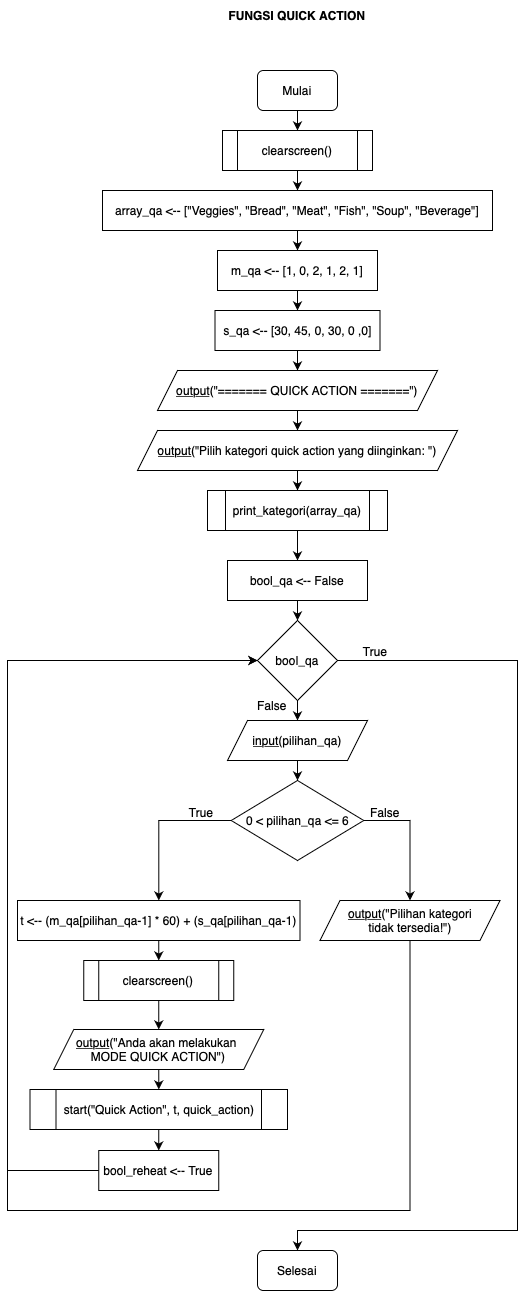
\includegraphics[scale=0.475]{QuickAction.png}}
    \caption{Flowchart Fungsi Quick Action}
    \label{fig12}
\end{figure}

\begin{figure}[htbp]
    \centering
    \def\svgwidth{\columnwidth}
    \centerline{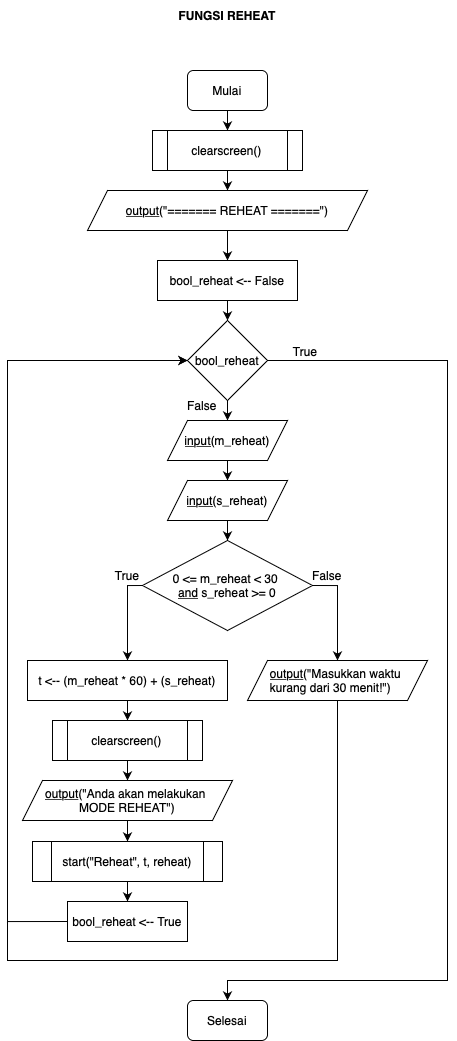
\includegraphics[scale=0.5]{Reheat.png}}
    \caption{Flowchart Fungsi Reheat}
    \label{fig13}
\end{figure}

\clearpage
\section{PENUTUP}

\subsection{Kesimpulan}
Berdasarkan pengembangan program microwave melalui pendekatan computational thinking ini, kita dapat menyimpulkan bahwa ilmu komputasi ini sangat bermanfaat dan mengambil peran dalam banyak hal,
termasuk dalam masalah di kehidupan sehari-hari. Pengembangan ilmu programming sangat memudahkan kehidupan manusia, sehingga manusia dapat beraktivitas dengan efektif dan efisien.
Contohnya, dalam program microwave ini, kita hanya perlu menentukan mode, waktu, dan suhu yang tepat, lalu menunggu beberapa waktu untuk proses, dan akhirnya kita dapat menikmati hasilnya secara langsung,
tanpa perlu berbuat banyak hal.

\subsection{Lesson Learned}
\begin{itemize}
    \item Menambah wawasan mengenai ilmu pengenalan komputasi, khususnya python.
    \item Mampu berpikir secara computational dan algorithmic kemudian mengaplikasikannya.
    \item Memahami bahwa programming memudahkan kehidupan manusia.
    \item Menambah wawasan mengenai penerapan array, conditional, fungsi, dan looping dalam benda elektronik, terutama microwave.
    \item Meningkatkan kerjasama antar anggota kelompok dalam pembuatan suatu program.
\end{itemize}

\section{Pembagian Tugas Dalam Kelompok}

\begin{enumerate}
\item[1.] Marcheline Fanni Hidayat Putri: Pprogam, Tugas 2, Flowchart
\item[2.] Angela Livia Arumsari: Program, Presentasi, Video
\item[3.] Miralistya Cahya Fatimah: Program, Tugas 1, Laporan
\end{enumerate}

\begin{thebibliography}{00}
\bibitem{b1} Panduan Penggunaan Sharp Microwave Oven [R-651ZS]. [online]. Available: https://manuals.plus/id/tajam/oven-microwave-tajam-r-manual-651zs
\bibitem{b2} Buku Instruksi dan Petunjuk Memasak MR87/MR89. [online]. Available: https://docplayer.info/72080362-Oven-microwave-buku-instruksi-dan-petunjuk-memasak-mr87-mr89-oven-2.html
\end{thebibliography}
\vspace{12pt}

\end{document}
